\documentclass{beamer}

% Packages.
\usepackage[english]{babel}
\usepackage{graphicx}
\usepackage{amsmath}
\usepackage{amssymb}
\usepackage{comment}
\usepackage[utf8]{inputenc}
\usepackage{lmodern}
\usepackage[T1]{fontenc}
\usepackage[nounderscore]{syntax}
\usepackage{microtype}
\usepackage{nameref}
\usepackage{ulem}

% Styling.
\setlength{\parskip}{1em}
\usetheme[style=plain,includehead=false,sidebar=true]{uu}
\setlength{\grammarindent}{6.5em}

% Title, subtitle, author and date.
\title{Grammatical Evolution Considered Harmful} %TODO
\subtitle{Evolutionary Computing 2014}
\author{Bert Massop, Simon Prins, Tom Tervoort}
\date{January 23, 2014}

% Macros.
\makeatletter
\newcommand*{\currentname}{\@currentlabelname}
\makeatother
\newcommand{\paper}[2]{\begin{centering}
\usebeamercolor[fg]{title}\usebeamerfont{title}#1\par
\bigskip\normalsize{}\usebeamercolor[fg]{normal text}\usebeamerfont{normal text}#2\par
\end{centering}}

\begin{document}

% Title page.
\begin{frame}
\titlepage
\end{frame}

\section{Grammatical Evolution}
\subsection{Introduction}
\begin{frame}
\frametitle{\currentname}
\begin{itemize}
\item Grammatical Evolution is \dots 
\item Introduced in paper Grammatical Evolution by Michael O’Neill et al.
\item Encode choices in grammar as array of binary integers.
\item Use standard bit flip mutation and one point crossover.
%TODO Add example?
\end{itemize}

\end{frame}

\subsection{Other techniques}
\begin{frame}
Genetic Programming:
\begin{itemize}
\item Uses tree representation.
\item Swap nodes in tree as crossover.
\end{itemize}
% Mention GP and compare.
\end{frame}



\section{Ms.\,Pac-Man controller}
\begin{frame}
\paper{Evolving a Ms.\,Pac-Man Controller Using Grammatical Evolution}{E. Galv\'an, J. Swafford, M. O'Neill, and A. Brabazon}
\end{frame}

\subsection{Goal}
\begin{frame}
\frametitle{\currentname}

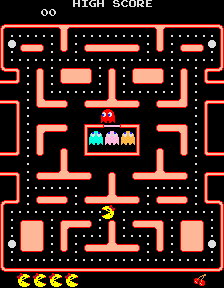
\includegraphics[scale=0.5]{Mspacman.png}
\begin{itemize}
\item Use GE to evolve rules.
\item Rules allow Ms. Pac-Man to maneuver through the maze.
\item Rules maximize score.
\end{itemize}
\end{frame}

\subsection{Experiment setup}
\begin{frame}
\frametitle{\currentname}
Record scores over 100 runs with one life and in one level.
Compare best evolved agent against:
\begin{itemize}
\item Random agent
\item Random non-reverse agent
\item Simple Pill Eater agent
\item Hand-coded agent
\end{itemize}
Against three different ghost teams.
\end{frame}

\subsection{Results}
\begin{frame}
\frametitle{\currentname}
%TODO insert table of scores.

\includegraphics[page=9, trim={3.5cm 10.5cm 3.5cm 3cm}, clip, scale=0.75]{PacMan_GE.pdf}


\end{frame}



\section{Super Mario Bros levels}
\begin{frame}
\paper{Evolving Levels for Super Mario Bros Using Grammatical Evolution}{N. Shaker, M. Nicolau, G. Yannakakis, J. Togelius, and M. O'Neill}
\end{frame}

\subsection{Goal}
\begin{frame}
\frametitle{\currentname}
\begin{itemize}
\item Evolve levels for Infinite Mario Bros using Grammatical Evolution.
\item To provide a framework for analyzing and comparing expressivity ranges of different generators.
\end{itemize}
\end{frame}

\subsection{Experiment setup}
\begin{frame}
\frametitle{\currentname}
Evolve level for Notch's Infinite Mario Bros game.\\
Compare against Notch's level generator and against an adapted version of that generator.\\
Use the following measures to compare them:
\begin{itemize}
\item Linearity
\item Density
\item Leniency
\item Compression Distance
\end{itemize}
\end{frame}

\subsection{Results}
\begin{frame}
\frametitle{\currentname}
\includegraphics[page=5, trim={11cm 15.5cm 1.5cm 8cm}, clip, scale=1.2]{Mario_GE.pdf}
\end{frame}



\section{Discussion}
\begin{frame}
\frametitle{Not all papers are created equal\dots}
\end{frame}

\begin{frame}
\only<1>{\paper{Evolving Levels for Super Mario Bros Using Grammatical Evolution}{N. Shaker, M. Nicolau, G. Yannakakis, J. Togelius, and M. O'Neill}}
\only<2>{\paper{Evolving Levels for \sout{Super} \textit{Infinite} Mario Bros Using Grammatical Evolution}{N. Shaker, M. Nicolau, G. Yannakakis, J. Togelius, and M. O'Neill}}
\end{frame}

\begin{frame}
\frametitle{A simple grammar}
\begin{grammar}
<prog>     ::= \synt{action} \synt{object} \hfill (0) \hspace{1em}
            \alt \lit*{if} \lit*(\synt{object} \lit*{is} \synt{property}\lit*)
              \\\lit*{\{} <prog> \lit*{\}} \hfill (1) \hspace{1em}

<object>   ::= \lit*{nuclear missile} \hfill (0) \hspace{1em}
            \alt \lit*{kitten} \hfill (1) \hspace{1em}

<property> ::= \lit*{dirty} \hfill (0) \hspace{1em}
            \alt \lit*{clean} \hfill (1) \hspace{1em}

<action>   ::= \lit*{clean} \hfill (0) \hspace{1em}
            \alt \lit*{launch} \hfill (1) \hspace{1em}
            \alt \lit*{look at} \hfill (2) \hspace{1em} \par
\end{grammar}
\end{frame}

\begin{frame}
\frametitle{Some sentences}
\framebox{\parbox{19em}{\scriptsize\color{black}
\begin{grammar}
<prog>     ::= \synt{action} \synt{object} \hfill (0) \hspace{1em}
            \alt \lit*{if} \lit*(\synt{object} \lit*{is} \synt{property}\lit*)
              \\\lit*{\{} <prog> \lit*{\}} \hfill (1) \hspace{1em}

<object>   ::= \lit*{nuclear missile} \hfill (0) \hspace{1em}
            \alt \lit*{kitten} \hfill (1) \hspace{1em}

<property> ::= \lit*{dirty} \hfill (0) \hspace{1em}
            \alt \lit*{clean} \hfill (1) \hspace{1em}

<action>   ::= \lit*{clean} \hfill (0) \hspace{1em}
            \alt \lit*{launch} \hfill (1) \hspace{1em}
            \alt \lit*{look at} \hfill (2) \hspace{1em} \par
\end{grammar}}}

\parbox[t][][t]{13em}{\textbf{1 7 4 4 6 3}
\\\texttt{if (kitten is dirty)
\\\{
\\\hspace*{2em}clean kitten
\\\}}
\\\textit{kitten happiness = 9}}
\parbox[t][][t]{13em}{\textbf{8 5 3}
\\\texttt{look at kitten\\\null\\\null\\}
\\\textit{kitten happiness = 7}}
\end{frame}

\begin{frame}
\frametitle{Genetic operator performance}
\framebox{\parbox[t][][t]{13em}{\textbf{1 7 4 4 6 3}
\\\texttt{if (kitten is dirty)
\\\{
\\\hspace*{2em}clean kitten
\\\}}
\\\textit{kitten happiness = 9}}
\parbox[t][][t]{9em}{\textbf{8 5 3}
\\\texttt{look at kitten\\\null\\\null\\}
\\\textit{kitten happiness~=~7}}}
\vfill


\visible<2->{\parbox[t][][t]{13em}{1 \textbf{7 4 4 6 3}
\\\textbf{8} 5 3
\visible<4->{
\\\texttt{launch nuclear missile}
\\\textit{kitten happiness = 0}}}
}
\visible<3->{\parbox[t][][t]{13em}{\sout{1} \textbf{7 4 4 6 3}
\\\textbf{2}
\visible<4->{
\\\texttt{launch nuclear missile}
\\\textit{kitten happiness = 0}}}
}
\end{frame}

\end{document}